\begin{figure*}[htb]
  \centering
  \begin{subfigure}[t]{0.33\textwidth}
    \centering
    \includegraphics[width=\textwidth]{figures/profile-mot.pdf}
    \caption{Pedestrian Detection}
    \label{fig:pd-profile}
  \end{subfigure}
  \hfill
  \begin{subfigure}[t]{0.33\textwidth}
    \centering
    \includegraphics[width=\textwidth]{figures/profile-darknet.pdf}
    \caption{Augmented Reality}
    \label{fig:ar-profile}
  \end{subfigure}
  \hfill
  \begin{subfigure}[t]{0.33\textwidth}
    \centering
    \includegraphics[width=\textwidth]{figures/profile-topk.pdf}
    \caption{Top-k}
    \label{fig:tk-profile}
  \end{subfigure}
  \caption{Application profiles of three applications. Each cross point
    indicates one configuration $c$'s performance $(B(c), A(c))$. All figures
    show the Pareto boundary as well as the performance if only one dimension is
    tuned.}
  \label{fig:all-profiles}
\end{figure*}

\newpage

\section{Evaluation}
\label{sec:evaluation}

In this section, we show our evaluations of \sysname{}. The results are
summarized as follows.

\begin{itemize}
\item[\autoref{sec:application-profiles}] \sysname{} generates Pareto-optimal
  profiles across multiple dimensions with precision
  (\autoref{fig:all-profiles}).
\item[\autoref{sec:online-profiling}] Our parallel and partial profiling enables
  fast online profiling with about 10\% GPU time (\autoref{fig:parallel},
  \autoref{fig:online-tricks}).
\item[\autoref{sec:runtime-adaptation}] At runtime, \sysname{} applications
  achieve sub-second latency and little accuracy drop
  (\autoref{fig:all-runtime}).
\item[\autoref{sec:multi-task-alloc}] \sysname{} profiles allow equal-accuracy
  bandwidth allocation among multiple streams (\autoref{fig:multitask}).
\end{itemize}

\subsection{Application Profiles}
\label{sec:application-profiles}

Our system learned the application profiles for all three applications using the
dataset specified in~\autoref{tab:apps}. We show the profiling results of all
configurations and the learned Pareto-optimal boundary
(\autoref{fig:all-profiles}). In addition, we highlight the configurations from
tune only one dimension. These profiles suggest the following:

\para{Large variation for bandwidth demand:} There is three to four orders of
magnitude of difference in their bandwidth requirements (note the x-axis is in
log scale). For PD and AR, the most expensive configuration transmits videos
with 1080p and 30FPS, using minimal quantization; it takes 230 mbps. In
constrast to the variation in bandwidth, there is a smaller variation in
accuracy. In PD, for example, even after the bandwidth is 1 mbps (less than 1\%
of the maximum), the accuracy is still above 75\%. This allows \sysname{}
applications running continuously with acceptable accuracy even under severe
network deterioration.

\para{Optimal configuration needs multiple dimensions.} We compare the
Pareto-optimal boundary with lines that indicates the performance of tuning one
knob. For PD and AR, the optimal configuration is only achieved with a
combination of tuning resolution, frame rate and quantizer. Tuning only one
dimension leads to sub-optimal performance. In Top-K, the Pareto-optimal is
mostly achieved with tuning \texttt{N}. While \texttt{T} doesn't contribute much
with this particular dataset, if another dataset is used with a different
distribution, we will see a different profile.

\para{Each dimension affects differently}. Within a single profile, we see how
different dimensions affect the bandwidth and accuracy differently. For PD,
tuning resolution (purple line) leads to a quicker accuracy drop in comparison
to tuning frame rate (green line). Across PD and AR, the same dimension has
different impact. Tuning resolution is less harmful in AR than PD; tuning frame
rate is more harmful in AR than PD. This echoes our initial observation that
application- and context-specfic strategy doesn't generalize
in~\autoref{sec:making-case-sys-approach}.

\para{Quantification with precision}. All the generated profiles come with
precise measures on how the configurations affect the bandwidth demand and
application accuracy. This saves developers from laboriously analyzing their
application to compute manual policies.

\newpage

\subsection{Profiling Efficiency and Online Profiling}
\label{sec:online-profiling}

This section focuses on the AR application as a case study.

\begin{figure}
  \centering
  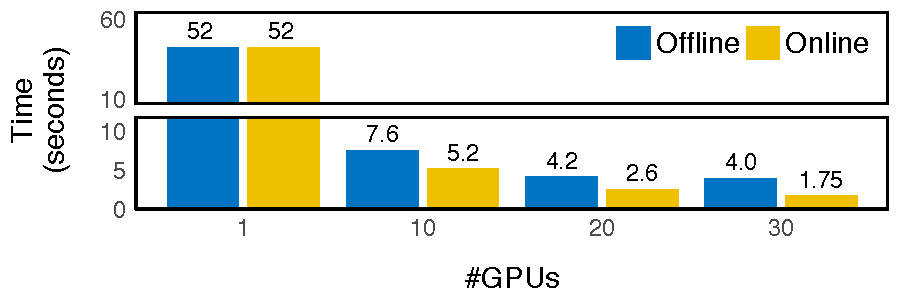
\includegraphics[width=0.8\columnwidth]{figures/parallel.pdf}
  \caption{Degradation-aware parallel scheduling}
  \label{fig:parallel}
\end{figure}

\para{Parallelism reduces the profiling time}. In AR, we have 216 configurations
to evaluate: 6 resolutions, 6 frame rates and 6 different quantizers. Processing
each frame with Yolo takes about 33 ms per frame. But different configurations
takes different amount of time. A configuration with 10FPS only needs to process
1/3 of the images of a configuration with 30FPS. In our experiments, the total
amortized processing time per frame is 1852 ms. When we perform the offline
profiling, we assign tasks randomly to each worker. While parallelism helps,
it's still often a suboptimal scheduling as two expensive configurations may be
assigned to the same worker. During the online profiling, we use the offline
profiling information to schedule tasks using the offline profiling.

\begin{figure}
  \centering
  \begin{subfigure}[t]{0.48\columnwidth}
    \centering
    \includegraphics[width=\textwidth]{figures/online1.pdf}
    \caption{Offline}
    \label{fig:offline}
  \end{subfigure}
  \hfill
  \begin{subfigure}[t]{0.48\columnwidth}
    \centering
    \includegraphics[width=\textwidth]{figures/online2.pdf}
    \caption{Online}
    \label{fig:online}
  \end{subfigure}
  \\
  \vspace{1.5em}
  \begin{subfigure}[t]{0.48\columnwidth}
    \includegraphics[width=\textwidth]{figures/online3.pdf}
    \caption{Online (Partial)}
    \label{fig:online-partial}
  \end{subfigure}
  \hfill
  \begin{subfigure}[t]{0.48\columnwidth}
    \includegraphics[width=\textwidth]{figures/online4.pdf}
    \caption{Online (Trigger)}
    \label{fig:online-trigger}
  \end{subfigure}
  \caption{Evaluation of various online profiling schemes. The accuracy across
    four schemes are similar (omitted).}
  \label{fig:online-tricks}
\end{figure}

\para{Online profiling address model drift}. First we show that the offline
learned model can fail to match the test data. The profile is generated against
a video clip of the office environment. Suppose there is 11 mbps available
bandwidth, according to the profile, the application should operate at a
configuration of 1280x720 resolution, 30FPS and a quantization factor of 20. We
run this configuration over a test video clip collected at the first author's
home. At about 100 seconds, the camera points out of the window to detect
objects on the street. Because of the scene change, the configuration fails to
predict the actual bandwidth demand. \autoref{fig:offline} shows the bandwidth
requirement over time; and the increase at 100 seconds is due to the data
change. To correct the misprediction, if we continuously run online profiling
and update the profile model, we will be able to capture the data distribution
change and predict the bandwidth demand more precisely (\autoref{fig:online}).

\para{Partial Profiling reduces profiling cost}. In practice, we only get holds
to a fraction of data. \autoref{fig:online-partial} evaluates the behavior if
only one third of the data is used for profiling. We notice there are two main
differences in comparison to \autoref{fig:online}. Between 80-100 seconds, it's
because of the limited data, hence an inaccurate profiling. At 110-140 seconds,
the profiling is not running, hence a delayed reaction.

\para{Trigger profiling is enough}. We trigger a full profiling if the bandwidth
estimation is off by 1 mbps or the accuracy is off by
10\%. \autoref{fig:online-trigger} shows that this is enough to track drastic
changes in the data distribution. Because a subset of all configurations can be
a significant saving, when we configure it with 5 profiling, the amortized cost
for each frame is 223 ms (~12\% of the GPU time)

%% Offline: 0
%% Online: 1 frame (1852.21 GPU * seconds)
%% Online (1/10)   (185.2 GPU * seconds)
%% Trigger         ( GPU * seconds)

\begin{table}[t]
  \centering
  \begin{tabular}{c|c|c|c}
    \hline
    offline & online & online (partial) & online (trigger) \\
    \hline
    0       & 1852 (ms)   & 617 (ms)              & 223 (ms) \\
    \hline
  \end{tabular}
  \caption{Online Profiling Time}
  \label{tab:online}
\end{table}

\begin{figure*}[!htb]
  \begin{subfigure}[t]{0.5\textwidth}
    \centering
    \includegraphics[width=\textwidth]{figures/runtime-legend.pdf}
  \end{subfigure}
  \\
  \vspace{1em}
  \begin{subfigure}[t]{0.3\textwidth}
    \centering
    \includegraphics[width=\textwidth]{figures/runtime-mot-verticle.pdf}
    \caption{Pedestrian Detection}
    \label{fig:pd-runtime}
  \end{subfigure}
  \hfill
  \begin{subfigure}[t]{0.3\textwidth}
    \centering
    \includegraphics[width=\textwidth]{figures/runtime-darknet-verticle.pdf}
    \caption{Augmented Reality}
    \label{fig:ar-runtime}
  \end{subfigure}
  \hfill
  \begin{subfigure}[t]{0.3\textwidth}
    \includegraphics[width=\textwidth]{figures/runtime-topk-verticle.pdf}
    \caption{Top-k}
    \label{fig:tk-runtime}
  \end{subfigure}
  \caption{Application profiles.}
  \label{fig:all-runtime}
\end{figure*}

\newpage

\subsection{Runtime Adaptation}
\label{sec:runtime-adaptation}

This section presents the evaluation of the runtime behavior of three
applications. We conduct controlled experiments using five geo-distributed
servers from Amazon EC2 (different AWS region). Four act as worker nodes
(\textit{t2.micro} instances) and one acts as the aggregation server
(\textit{m4.xlarge} instance). For each experiment, the worker nodes transmit
test data for about 10 mins. We measure three aspects of the system: throughput,
latency and application accuracy.

We compare \sysname{} applications with baseline applications built with vanilla
TCP and UDP. Notice that the raw data streams are prohibitively large (230 mbps
for video streams). For a fair comparison, we pick a reasonable configuration as
the maximum rate for the baseline applications.

During the experiment session, we use Linux \texttt{tc} utility with
HTB~\cite{lartc} to adjust outgoing bandwidth to experiment with network
resource variation. At time 200 seconds, we impose the first traffic shaping. At
time 380 seconds, we impose a more severe shaping. At time 440 seconds, we clear
all the traffic shaping. Because of the different capacity of any pair-wise
connection, we always have a 25mbps cap for all PD and AR and 2.5 mbps for
TK. When evaluating UDP traffic, we use \texttt{netem} to emulate the packet
loss behavior with out-of-order delivery.

The results are shown in \autoref{fig:all-runtime}. Throughput figures reflect
the effect of our traffic shaping. Notice that after the traffic shaping stops,
TCP has a ``catch-up'' phase where it's sending all the queued items as fast as
possible (hitting the cap we set). Because of the queuing during the shaping
period, TCP suffers from an increased latency (as seen in the latency
figures). But the data is maintained at high fidelity in TCP, so the accuracy is
always high. For UDP, the latencies are constant. But during the phase of
traffic shaping, packet drop leads to drastic accuracy drop. In both PD and AR,
the accuracy are almost 0\%. For TK, it's below 50\% and getting worse in
between 380 and 440.

\para{\sysname{}'s adaptation achieves low latency and high accuracy}. We
achieve worse-case sub-second latency for PD and AR and 5 seconds latency for
TK. Because TK aggregates data every seconds, the queued object and the react is
at a granularity of at least 1 seconds. We also guarantee a relatively high
accuracy with across all applications in the face of bandwidth degradation.

\newpage

\subsection{Resource Allocation and Multitask Fairness}
\label{sec:multi-task-alloc}

We evaluate the resource allocation and multitask fairness with an example of
the pedestrian detection and augmented reality running along the same link. Both
applications starts with sufficient bandwidth. At 60 seconds, we start traffic
shaping to limit the total bandwidth at 6 mbps. With a resource fair
allocation~\autoref{fig:eq-bw}, PD runs with a higher accuracy (85\%) while AR
runs at (77\%). If we enable accuracy fairness, the resource allocation will
choose configurations that maximize the minimal accuracy, leading to both
operate at about 80\% accuracy~\autoref{fig:eq-acc}.

\begin{figure}
  \begin{subfigure}[t]{0.8\columnwidth}
    \centering
    \includegraphics[width=\textwidth]{figures/multitask-legend.pdf}
  \end{subfigure}
  \\
  \vspace{1em}
  \begin{subfigure}[t]{0.49\columnwidth}
    \centering
    \includegraphics[width=\textwidth]{figures/multitask-eq-bw.pdf}
    \caption{Resource Fairness}
    \label{fig:eq-bw}
  \end{subfigure}
  \hfill
  \begin{subfigure}[t]{0.49\columnwidth}
    \centering
    \includegraphics[width=\textwidth]{figures/multitask-eq-acc.pdf}
    \caption{Utility Fairness}
    \label{fig:eq-acc}
  \end{subfigure}
  \caption{Comparison between different schemes of resource allocations:
    resource fairness and utility fairness.}
  \label{fig:multitask}
\end{figure}

\newpage

%%% Local Variables:
%%% mode: latex
%%% TeX-master: "sosp17"
%%% End:
